\section{Постановка задачи}

Рассмотрим задачу классификации на $K$ классов:
$$\mathfrak{D}  = \{(\bold{x}_i, y_i)\}_{i=1}^{m},\; \bold{x}_i \in \mathbb{R}^n,\; y_i \in \mathbb{Y}  = \{1, \dots, K\},$$
где $\mathfrak{D}$ это доступная выборка объектов, $y_i$ --- целевая переменная, \\
а $\bold{x}_i$ --- данные, описывающие объект, взятые из распределения $p(\bold{x})$.

В задаче дистилляции нам необходима кроме обучаемой модели, так называемого ученика, еще модель учителя,
которая уже предобучена на такой же задаче, и параметры которой не меняются в процессе обучения.
Пропуская входные данные $\bold{x}$ через модель, мы можем после каждого слоя получить его активации.
Обозначим активации после $i$-го слоя модели учителя как $\bold{t}_i$, а активации после $j$-го слоя модели ученика как $\bold{s}_j$.

Взаимная информация \cite{Ahn_2019_CVPR} пары $(\bold{t}, \bold{s})$ определена как:
$$ I(\bold{t}; \bold{s}) = H(\bold{t}) - H(\bold{t} | \bold{s}) =  -\mathbb{E}_{\bold{t}}[\log{p(\bold{t})}] + \mathbb{E}_{\bold{t},\bold{s}}[\log{p(\bold{t}|\bold{s})}],$$
где энтропия $H(\bold{t})$ и условная энтропия $H(\bold{t}|\bold{s})$ получены из совместного распределения $p(\bold{t},\bold{s})$.
Определение $I(\bold{t}; \bold{s})$ можно понимать, как уменьшение неопределенности в знаниях учителя, которые закодированны в его слое $\bold{t}$,
когда известен слой $\bold{s}$ ученика.

Теперь, можем определить функцию потерь для модели ученика, минимизируя которую ученик будет не только обучаться для задачи классификации,
но и будет максимизироваться взаимная информация между слоями учителя и ученика:
$$\mathcal{L} = \beta \mathcal{L}_\text{CE} - (1 - \beta){\sum_{i=1}^T \sum_{j=1}^S \lambda_{i, j}I(\bold{t}_{i}, \bold{s}_{j})},$$
где $\mathcal{L}_\text{CE}$ --- кросс-энтропия, $T$ --- количество слоёв учителя, $S$ --- количество слоёв ученика, $\beta \in (0;1)$ --- гиперпараметр,
отвечающий за баланс между минимизацией кросс-энтропии и максимизацией взаимной информации между слоями учителя и ученика, $\lambda_{i, j} \in [0;1]$ ---
гиперпараметр, отвечающий за важность связи $i$-го слоя учителя и $j$-го слоя ученика.

\begin{figure}[!htbp]
    \centering
    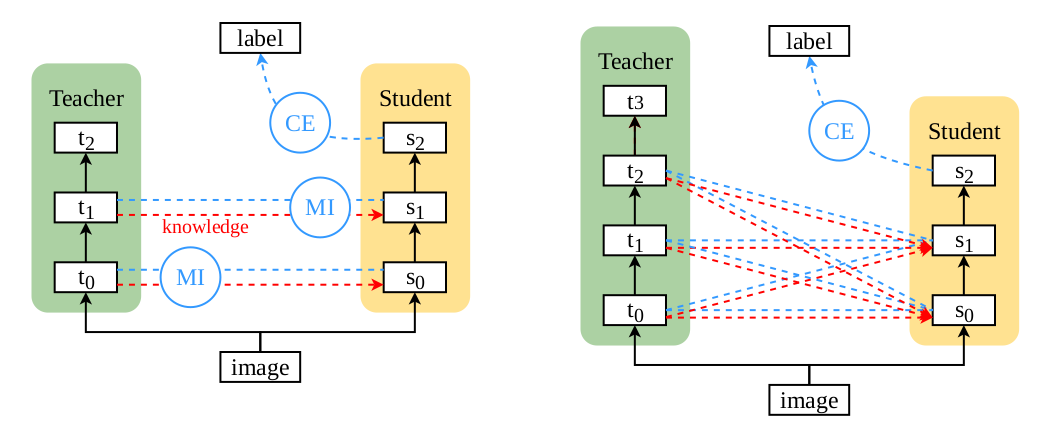
\includegraphics[width=0.9\textwidth]{method_scheme.png}
    \caption{Схема метода дистилляции Sungsoo Ahn \cite{Ahn_2019_CVPR} (слева) и предлагаемого нами метода (справа)}
    \label{fig:method_scheme}
\end{figure}

Схема нашего метода, в сравнении с уже упомянутым методом Sungsoo Ahn\cite{Ahn_2019_CVPR}, изображена на рисунке \ref{fig:method_scheme}.
